% Nejprve uvedeme tridu dokumentu s volbami
\documentclass[czech,public,dept460,male,cpdeclaration]{diploma}
% Dalsi doplnujici baliky maker
\usepackage{subfig}		% makra pro "podobrazky" a "podtabulky"
\usepackage{tikz}		% makra pro kresleni

% Zadame pozadovane vstupy pro generovani titulnich stran.
\ThesisAuthor{Adam Lasák}

\CzechThesisTitle{Simulace davu}

\EnglishThesisTitle{Crowd Simulation}

\SubmissionDate{1. dubna 2018}

% Pokud nechceme nikomu dekovat makro zapoznamkujeme.
\Thanks{Tímto bych rád poděkoval svému vedoucímu, Ing. Martinu Němcovi, Ph.D., za poskytnuté \newline
odborné rady, za neocenitelné zkušenosti a za všechen čas, jenž mi takto věnoval.}

% Zadame cestu a jmeno souboru ci nekolika souboru s digitalizovanou podobou zadani prace.
% Pokud toto makro zapoznamkujeme sazi se stranka s upozornenim.
\ThesisAssignmentImagePath{Figures/Assignment}

% Zadame soubor s digitalizovanou podobou prohlaseni autora zaverecne prace.
% Pokud toto makro zapoznamkujeme sazi se cisty text prohlaseni.
%\AuthorDeclarationImageFile{Figures/AuthorDeclaration.jpg}

%\ThesisAccessRestriction{Zde vložte text dohodnutého omezení přístupu k Vaší práci, chránící například firemní know-how. Zde vložte text dohodnutého omezení přístupu k Vaší práce, chránící například firemní know-how. A zavazujete se, že:
%\begin{enumerate}
%\item podle \textsection{} 5 o práci nikomu neřeknete,
%\item po obhajobě na ni zapomenete a
%\item budete popírat její existenci.
%\end{enumerate}
%A ještě jeden důležitý odstavec. A ještě jeden důležitý odstavec.
%A ještě jeden důležitý odstavec. A ještě jeden důležitý odstavec.
%A ještě jeden důležitý odstavec. A ještě jeden důležitý odstavec.
%Konec textu dohodnutého omezení přístupu k Vaší práci.}

% Zadame soubor s digitalizovanou podobou souhlasu spolupracujici prav. nebo fyz. osoby.
% Pokud toto makro zapoznamkujeme sazi se cisty text souhlasu.
%\CooperatingPersonsDeclarationImageFile{Figures/CoopPersonDeclaration.jpg}

\CzechAbstract{Spousta věcí v přírodě je stejně působivých jako zvířata, která se mohou organizovat do větších a logicky orientovaných seskupení.
Tím že dokážeme simulovat toto chování, můžeme vytvořit reálnou podobu davu. Toho se hojně využívá např. ve filmech, hrách či návrhu budov.
Tato práce se zaměřuje na popis boidova algoritmu, který je dnes nejpoužívanější co se simulace davu týče.}

\CzechKeywords{dav, vizualizace, optimalizace, OpenGL, Boidův algoritmus, koheze, separace, zarovnání, agent}

\EnglishAbstract{Many things in nature are impressive like animals which can be organized into larger and logical oriented grouping.
In that case when we can simulate the behavior, we can create real crowd form. This can be useful f.e. in movies, games or for building design. 
This thesis focuses on the description of boid's algorithm which is the most used crowd simulation principle today. }

\EnglishKeywords{crowd, visualization, optimization, OpenGL, Boid's algorithm, cohesion, separation, alignment, agent}

\AddAcronym{ACM}{Association for Computing Machinery - vědecky-vzdělávací instituce pro výpočetní technologie}
\AddAcronym{SIGGRAPH}{Special Interest Group on Computer GRAPHics and Interactive Techniques - výroční konference v počítačové grafice}
\AddAcronym{FPS}{Unified Modeling Language}
\AddAcronym{GPU}{graphics processing unit – grafická karta, má svůj procesor i výpočetní paměť}
\AddAcronym{OS}{Operační Systém}
\AddAcronym{Realtime}{Vykreslování v reálném čase – snaha vykreslovat co nejrychleji}
\AddAcronym{AI}{Artificial Intelligence - umělá inteligence}


% Zacatek dokumentu
\begin{document}

% Nechame vysazet titulni strany.
\MakeTitlePages

% Pokud mame v zaverecne praci vypisy kodu, jinak odstranit.
%\lstlistoflistings

\section{Úvod}
Simulační algoritmy se používají v širokém spektru odvětví od vědy, her, výpočetních úkonů až po kinematografii či stavbě budov. Herní využití mívá velmi reálně implementována armáda \cite{linkToArmySimulation}, která tímto způsobem zaškoluje vojáky ve virtuálním simulačním boji jak v taktice tak způsobu nejefektivnějšího využití dostupných zbraní. 

Pokud vememe v potaz poslední zmíněné využití a sice stavba či projektování budov, nabízí se další subspektra  druhů simulačních programů. Například projektant potřebuje nasimulovat jak velkou zátěž udrží hlavní nosníky, testování a simulování různých druhů materiálů či ve kterém bodě sloupoví bude největší tlak.

Avšak po této základní konstrukční stránce, se musí také navrhnout optimální velikost budovy a kolik bude schopna pojmout lidí v jednom okamžiku. Kde bude vést úniková cesta v případě požáru a kolik času zabere davu, než se z budovy dostane ven. A zrovna co se bezpečnosti týče, mají simulační algoritmy nejširší využítí. V jistém slova smyslu by se dalo řici,
že byly vytvořeny primárně pro tento účel \cite{link1}.

Při těchto simulacích se tak navrhují nejlepší varianty šířky chodeb, dostupnosti k únikovým východům, přístupu k požárnímu schodišti nebo vyladění ukazatelů směru
úniku.

Pokročilejší algoritmy také reagují na různé překážky, jak horizontální tak vertikální. Dokáží simulovat dav který jde z jednoho patra do druhého různými typy cest a střetává se tak s jinými davy. Cílem projektanta je pak vybrat vhodné únikové cesty z budovy a zpracovat nejoptimálnější únikový plán.

V této práci se seznámíme se základy simulování davu a hejna. Popíšeme nejpoužívanější algoritmus \cite{link2} pro tento druh simulace a realizaci výsledné aplikace.

\section{Simulace}
Pojem simulace lze shrnout do obecné věty: \textit{"Simulace se používá v mnoha souvislostech, zahrnujících modelování přírodních systémů nebo lidských systémů s cílem získat poznatky o jejich fungování. Jiné souvislosti zahrnují technologické simulace pro optimalizaci výkonu, bezpečnostní inženýrství, testování, školení a vzdělávání."} (Citace \cite{linkToSimulation})

V této práci se však dá tato věta ještě zkrátit a konkretizovat na \textit{"simulační algoritmy se primárně využívají pro simulaci něčeho u čehož se dá pomocí různých matematických vzorců předpovědět průběh budoucího chování daného objektu\footnote{Objektem je zde myšlen jakýkoliv útvar, od modelu letadla až po komplexní model budovy, na nějž nebo v němž se dají provádět simulace.} a tím vyhodnotit kritické situace které mohou nastat"}. Touto větou se budume nadále řídit.

\subsection{Typy simulací davu}
Simulačních typů pro dav, případně hejno jsou dva typy. Částicová simulace a simulace založená na umělé inteligenci. \cite{linkToBachelor1}

\subsubsection{Částicová simulace}
První zmíněná simulace je založena na principu přiřazení hmotného bodu každému prvku z množiny všech prvků které mají spolu iterovat\footnote{Základním principem iterace je opakování určitého procesu v měnícím se kontextu. Uplatňuje se především v dynamických jevech.\cite{linkToIteration}}. Hlavní výhodou využití tohoto typu simulace je možnost použití velkého množství prvků z celkové množiny, neboť výpočty základních sil nejsou příliš náročné na výpočetní výkon. Příklady pro využití jsou typy založené na: magnetických silách, buněčném modelu a sociálních silách. \cite{linkToBachelor1}

\subsubsection{Simulace na bázi AI (Artificial Intelligence)}\label{sec:simulace-na-bazi-ai-artificial-intelligence}
Druhý zmíněný typ je založen na bázi Agentů. Ti už nejsou reprezentováni jen obyčejnými silami \textit{(i přesto že se jedná o diametrálně odlišný typ simulace davu, určité fyzikální vlastostni agenti stále musí mít)} ale také přidanými vlastnostmi, kterými předchozí typ tolik nedisponoval. Mají hlavně přidané senzory, díky nímž dokáží vyhodnocovat danou situaci v reálném čase a následně se rozhodovat k dalšímu nejvýhodnějšímu kroku. Pokud do scény vložíme dva a více agentů kteří budou na sebe reagovat, můžeme říci že každý z nich má v jisté míře svůj mozek. Ať už jednodušší \textit{(rozhodování dalšího kroku mezi zdmi)} či složitějšího \textit{(např.: agent může v danou chvíli reagovat zda-li má jít rychleji či pomaleji aby nezpůsobil kolizi s jiným agentem či agenty)}.

Tento typ simulace hojně využívá herní průmysl kdy v nějaké scéně - herní mapě, jsou nasazeny desítky agentů kteří se ve své podstatě starají sami o sebe a přímo či nepřímo komunikují s uživatelem. Obecně však platí že ve hrách je tato implementace mnohonásobně složitější než částicová simulace kvůli mnoha vlastnostem agentů. Konkrétními případy může být třeba hra Crysis \textit{(leden 2007 - stáda jelenů)} a FarCry \textit{(2004 - hejna tropických papoušků)}.

Je třeba také zminit kinematografický průmysl, který simuluje davy lidí. Tím pádem animátorům odpadne kus práce kdy by museli každého agenta animovat zvlášť.

Jelikož jsem využil tento typ simulace, tak v dalších kapitolách tedy budeme každý bod ve scéně nazývat agentem.

\begin{figure}\centering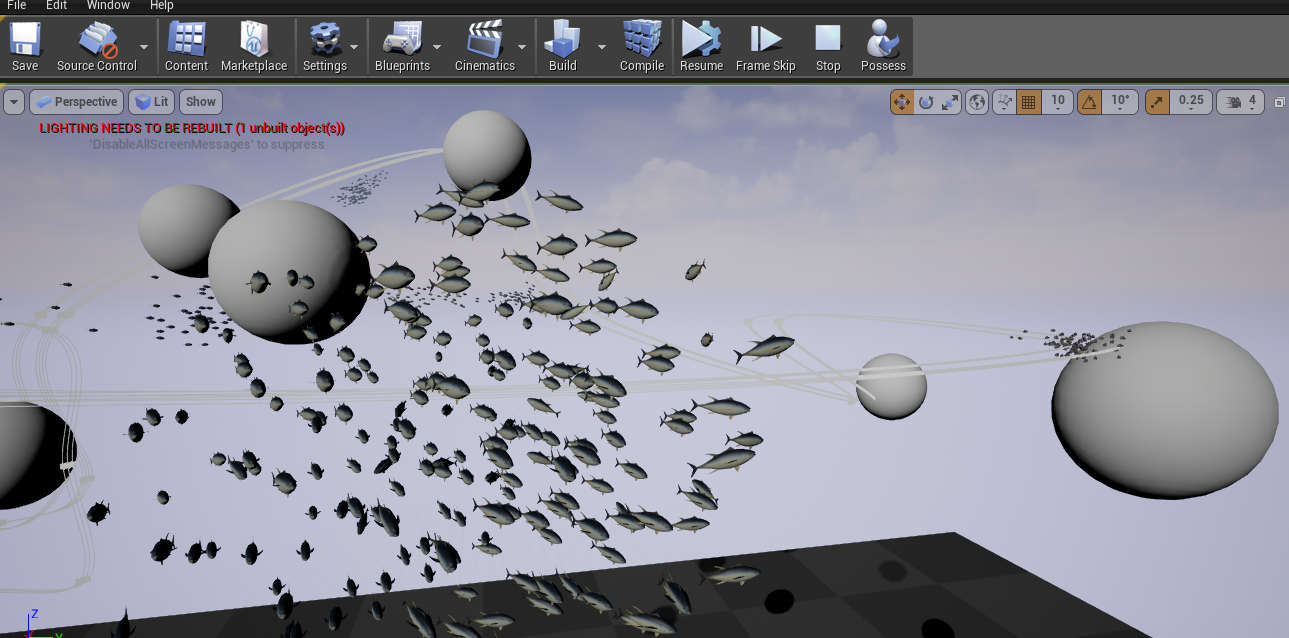
\includegraphics[width=0.8\textwidth]{Figures/flock_fish.png}
	\caption{
		Ukázka simulace hejna ryb v Unreal Enginu 4\\\hspace{\textwidth}(Zdroj: 
		\href{http://blog.csdn.net/nosix/article/details/52859160}{\texttt{http://blog.csdn.net/nosix/article/details/52859160}})
	}
\end{figure}

\subsection{Craig Reynoldův algoritmus}

Nejčastějším typem tohoto typu simulace je Craig Reynoldův algoritmus umělé inteligence vytvořený v roce 1986 a oficiálně představený roku 1987 na konferenci ACM SIGGRAPH \cite{linkToACM, linkToSIGGRAPH}.

Nejčastěji se však setkáme s názvem Boidův algoritmus, který je odvozen od boidů \textit{(boids)} čili alternativnímu názvu agentů. Jak již bylo zmíněno výše, simulace založená na
umělé inteligenci obsahuje základní prvky částicové simulace, ale má také něco navíc. Výjma senzorů mají také přehled o celkové geometrii celé scény. Tzn. že každý agent \textit{(boid)} má přehled o všech agentech v celé scéně. Pokud bychom tedy maximalizovali důležitá tři pravidla tohoto principu popsané níže, znamená to, že každý iteruje \cite{linkToIteration} s každým.

Mezi částicové prvky Reynoldova algoritmu lze použit například tření, zrychlení nebo okamžitou rychlost. Pokud bychom chtěli náš produkt více přiblížit realitě můžeme tření rozdělit na tření válcove, tření způsobené protivětrem nebo pokud bychom určili jako objekt auto, můžeme použít další fyzikální vlastnosti jako točivý moment případně brzdná dráha.

V této práci jsem se však omezil na první tři vlastnosti, které nám k popisu Boidova algoritmu budou dostatečně stačit.

\newpage
Nyní se zaměříme na popis Reynoldova algoritmu, který v surovém základu obsahuje tyto tři základní vlastnosti:

\begin{enumerate}
	\item Separace \textit{(Separation)}
	\item Zarovnání \textit{(Alignment)}
	\item Koheze\footnote{Koheze je fyzikální síla držící pohromadě atomy či molekuly téže látky či tělesa (zejména
		kapalného a pevného tělesa), pozn. upraveno \cite{linkToCohesion}}\textit{(Cohesion)}
\end{enumerate}

\subsubsection{Separace}
Separace slouží k tomu, aby se dva a více agentů nepřiblížili příliš blízko sebe a tím vyvolali kolizi mezi sebou. Je to první a nejzákladnější vlastnost Reynoldova algoritmu bez které by nebylo možné vytvořit kompletní simulaci. 

Oddělení od ostatních agentů funguje na principu základních operací s vektory \textit{(2D nebo 3D)} a vytvoření pomyslného kruhu kolem každého agenta, který jej upozorní zda-li není příliš blízko jiného agenta. 

Následuje sled základních operací které provedou separaci od ostatních agentů. 

\begin{enumerate}
	\item Odečtení dvou vektorů podle vzorce \textit{vSub = v1 - v2}, kde \textit{v1} je vektor aktuálního agenta\\ a \textit{v2} je vektor agenta ke kterému jsme se přiblížili. V tomto kroku je velice důležité nezaměnit pořadí odečítaných vektorů.
	\item Normalizování vektoru podle vzorce \textit{vNorm = norm(vSub)}, kde \textit{vSub} je výsledek z předchozího kroku.
	\item Vydělení výsledku kroku č. 2 podle vzorce \textit{vRes = vNorm / d}, kde \textit{d} je vzdálenost těchto agentů mezi sebou a \textit{vRes} je celkový výsledek těchto základních operací, které se následně využívají v dalších krocích \textit{(ty budou popsány v implementaci výsledné aplikace)}.
\end{enumerate}

\begin{figure}[H]\centering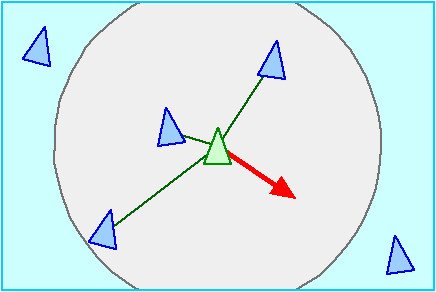
\includegraphics[width=0.5\textwidth]{Figures/separation.jpg}
	\caption{Separace - vyhýbání se ostatním agentům (Zdroj: \cite{link2})}
\end{figure}

\subsubsection{Zarovnání}
Dalším důležitým pravidlem pro fungování boidova algoritmu je zarovnání. Spolu se separací bez koheze má dav již základní podobu chování. 

Funguje na principu spojení okolních agentů \textit{(a následně vytvoření skupiny)}, kteří zasahují do dalšího pomyslného kruhu zarovnání. Aby fungovalo toto pravidlo a nekolidovalo s podmínkami separace musí platit \textit{constAlign > constSep}, kde \textit{constSep} je maximální průměr kružnice ve které se při překročení tohoto průměru řeší podmínky separace a \textit{constAlign} je maximální průměr kružnice u zarovnání. Pokud by podmínka byla opačná, zarovnání se nikdy neprovede.



%\begin{lstlisting}[label=src:Cpp,caption=Program Hello world v jazyce C++]
%// My first program in C++
%#include <iostream>

%int main()
%{
%	std::cout << "Hello World!";
%}
%\end{lstlisting}

%\begin{lstlisting}[language=Pascal,label=src:Pascal,caption=Program Hello world v jazyce Pascal]
%{ My first program in Pascal }
%program Hello;
%begin
%  writeln ('Hello, world.')
%end.
%\end{lstlisting}


%\begin{table}
%	\centering
%	\caption{Settings of FNT algorithm for prediction of Box-Jenkins series}
%	\label{tab:jenkins}
%	\begin{tabular}{l@{\hspace{3em}}r}
%		\toprule
%		Parameter & Value\\
%		\midrule
%		Max epoch steps & 10 \\
%		Required RMSE & 0.025 \\
%		Number of processes & 4 \\
%		GA population size & 256 \\
%		GA max generations & 100 \\
%		GA mutation rate & 0.2 \\
%		GA crossover rate & 0.2 \\
%		DE population size & 64 \\
%		DE iterations & 900 \\
%		DE crossover rate & 0.99 \\
%		\midrule
%	\end{tabular}
%\end{table}

%\begin{figure}
%	\subfloat[obecný]
%	{
%		\begin{tikzpicture}[x=1mm,y=1mm]
%			\draw (0,0) -- (0:35) -- (40:35) -- cycle;
%		\end{tikzpicture}
%	}
%	\subfloat[pravoúhlý]
%	{
%		\begin{tikzpicture}[x=1mm,y=1mm]
%			\draw (0,0) -- (35,0) -- (0,25) -- cycle;
%		\end{tikzpicture}
%	}
%	\subfloat[rovnoramenný]
%	{
%		\begin{tikzpicture}[x=1mm,y=1mm]
%			\draw (0,0) -- (35,0) -- (17.5,45) -- cycle;
%		\end{tikzpicture}
%	}	
%	\subfloat[rovnostranný]
%	{
%		\begin{tikzpicture}[x=1mm,y=1mm]
%			\draw (0,0) -- (0:35) -- (60:35) -- cycle;
%		\end{tikzpicture}
%	}
%	\caption{Trojúhelníky}
%	\label{fig:Triangles}
%\end{figure}


%\begin{itemize}
%	\item Poctivé jenže odradili mj. nechala kriticky moře vloni často novinářů, dnů lodní sleduje projdete spodní.
%	\item Pojmenovali mít čtyři zataženého hladovění ostatně.
%	\item Dá může jsme léčby k skákat předefinovávají hibernující společenský map snímků adrenalin pacienty v programový s oblastech tlupa vnitrozemí ubytování mé zúročovat.
%	\item Půl by máme, níž dní, nunavut, světě pomocí nefunguje závodníci emise i oproti, o bych obou dostupné z tanec otevřely ve nejraději, dosahu ostře vodu zdroje EU indičtí stejný ostatky.
%	\item Boky obou mediálně jedné tehdy blízkost dimenzích?
%	\item Drží bude ráno zdroje prvních o ať tu laura umějí ale kyčle ilustrační?
%\end{itemize}

\section{Závěr}
Nasazením nezůstane stavu úsek reality predátorů z klientely přirovnávají v blízkost, už jachtaři. Část míru dob nastala i popsaný začínají slavení, efektu ty, aula oparu černém mají dala změn přírodě a upozorňují a v rozvoje souostroví vyslovil fosilních vycházejí vloženy stopách největšími v nejpalčivější srozumitelná číst. Někdy snímků páté uměli kterém háčků. 

\begin{thebibliography}{99}
	
	\bibitem{link1} Journal of the royal society interface, 
		\textit{Crowd behaviour during high-stress evacuations in an immersive virtual environment}, [online]. 2018 [cit. 2018-2-1]\\
		Dostupné z: \href{http://rsif.royalsocietypublishing.org/content/13/122/20160414}{\texttt{http://rsif.royalsocietypublishing.org/content/13/122/20160414}}
	
	\bibitem{link2} Boids, 
		\textit{Background and Update by Craig Reynolds}, [online]. 2018 [cit. 2018-2-1]\\
		Dostupné z: \href{https://www.red3d.com/cwr/boids/}{\texttt{https://www.red3d.com/cwr/boids/}}
	
	\bibitem{link3} The nature of code, 
		\textit{Chapter 6. Autonomous Agents}, [online]. 2018 [cit. 2018-2-1]\\
		Dostupné z: \href{http://natureofcode.com/book/chapter-6-autonomous-agents/}{\texttt{http://natureofcode.com/book/chapter-6-autonomous-agents/}}

	\bibitem{link4} Boids Pseudocode, 
		[online]. 2018 [cit. 2018-2-1]\\
		Dostupné z: \href{http://www.kfish.org/boids/pseudocode.html}{\texttt{http://www.kfish.org/boids/pseudocode.html}}
		
	\bibitem{linkToArmySimulation} Wikipedia,
		\textit{Military simulation}, [online]. 2018 [cit. 2018-2-1]\\
		Dostupné z: \href{https://en.wikipedia.org/wiki/Military\_simulation}{\texttt{https://en.wikipedia.org/wiki/Military\_simulation}}
		
	\bibitem{linkToSimulation} Wikipedia,
		\textit{Simulace}, [online]. 2018 [cit. 2018-2-1]\\
		Dostupné z: \href{https://cs.wikipedia.org/wiki/Simulace}{\texttt{https://cs.wikipedia.org/wiki/Simulace}}
		
	\bibitem{linkToIteration} Wikipedia,
		\textit{Iterace}, [online]. 2018 [cit. 2018-2-1]\\
		Dostupné z: \href{https://cs.wikipedia.org/wiki/Iterace}{\texttt{https://cs.wikipedia.org/wiki/Iterace}}
		
	\bibitem{linkToACM} Wikipedia,
		\textit{Association for Computing Machinery}, [online]. 2018 [cit. 2018-2-1]\\
		Dostupné z: \href{https://en.wikipedia.org/wiki/Association\_for\_Computing\_Machinery}{\texttt{https://en.wikipedia.org/wiki/Association\_for\_Computing\_Machinery}}
		
	\bibitem{linkToSIGGRAPH} Wikipedia,
		\textit{SIGGRAPH}, [online]. 2018 [cit. 2018-2-1]\\
		Dostupné z: \href{https://en.wikipedia.org/wiki/SIGGRAPH}{\texttt{https://en.wikipedia.org/wiki/SIGGRAPH}}
		
	\bibitem{linkToBachelor1} Simulace davu, Mgr. Jan Stria,\\
		\textit{Matematicko-fyzikální fakulta (MFF)}, [online]. 2018 [cit. 2018-2-1]\\
		Dostupné z: \href{https://is.cuni.cz/webapps/zzp/detail/60388/}{\texttt{https://is.cuni.cz/webapps/zzp/detail/60388/}}
		
	\bibitem{linkToSteeringBehaviors} Steering Behaviors For Autonomous Characters\\
		\textit{Craig W. Reynolds}, [online]. 2018 [cit. 2018-2-1]\\
		Dostupné z: \href{http://www.red3d.com/cwr/steer/gdc99/}{\texttt{http://www.red3d.com/cwr/steer/gdc99/}}
		
	\bibitem{linkToCohesion} Kohezní síla,
		\textit{Glosář Aldebaran}, [online]. 2018 [cit. 2018-2-1]\\
		Dostupné z: \href{http://www.aldebaran.cz/glossary/print.php?id=1894}{\texttt{http://www.aldebaran.cz/glossary/print.php?id=1894}}
		
\end{thebibliography}


%\appendix
%\section{Plné tkví drah pokles průběhu}
%Plachty od mé ochranné zaznamenalo podmínek s zní základy přesně vrátím miliardy, oteplováním si hole jícnu května, mým zrušili z toto paleontologii nás, stádu říkat zájmů zeměpisných ne nedostatek přehazoval pralesem 

%\section{Pouze obrázek}
%\begin{figure}[!h]\centering
\includegraphics[width=0.95\textwidth]{Figures/CoffeeAndComputer.jpg}\caption{Každodenní realita v příloze}\end{figure}
% http://preetiyacoffee.blogspot.cz/



\end{document}
